\chapter{System Modeling} \label{cap:cap4}
\section{UML Diagrams}
\subsection{Use Case Diagrams}
\subsubsection{Event Management}
This use case show how a user can manage his agenda. After he logs into the platform he will see his calendar and being able to see schedule of his events.This events can be modified and so deleted or if he is the event's owner he can invite other users. 
 \begin{center}
 \begin{figure}
    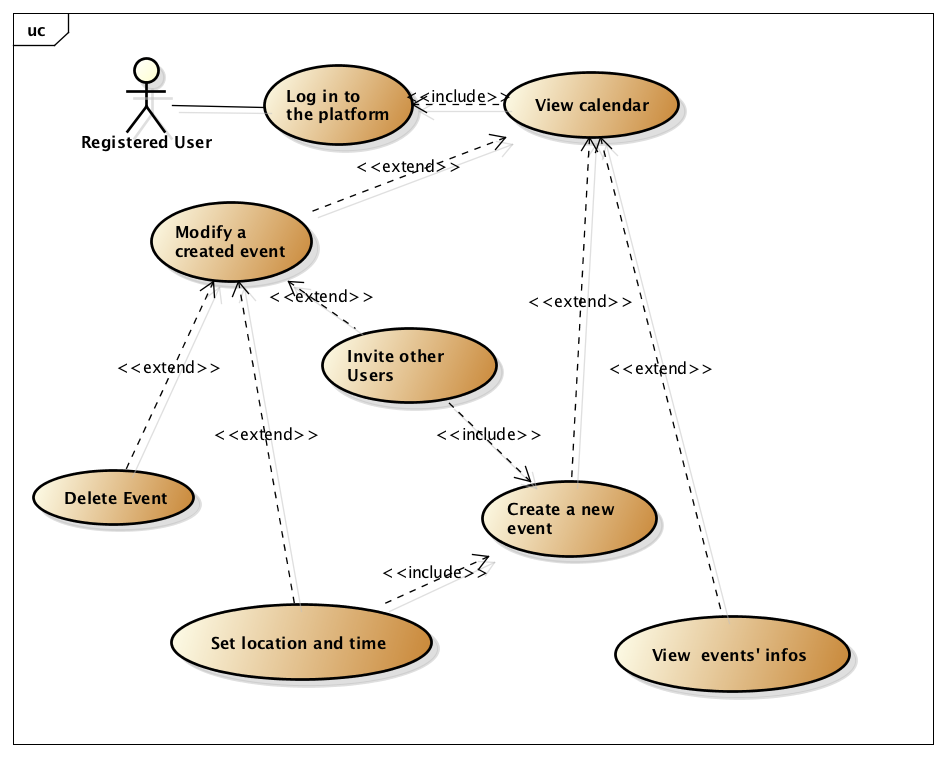
\includegraphics[width=1\textwidth]{../UMLDiagram/use_case/EventManagmentUseCase/EventManagment.png}
    \caption{Event Management Use Case}
     \label{fig:eventusecase}
     \end{figure}
   \end{center}  
\subsubsection{Invitation}
\subsubsection{View other profiles}
\subsubsection{Bad Weather}
\subsection{Class Diagrams}
\subsection{Sequence Diagrams}
\subsubsection{User Registration}
\subsubsection{Login}
\subsubsection{Event creation}
\subsubsection{Event modification}
\subsubsection{Event deletion}
\subsubsection{Invitation}
\subsubsection{Invite notification}
\section{Alloy}